\chapter{Metodi di Anomaly Detection}
\label{chap:methods}

\section{Learning Models}
I learning models sono algoritmi che utilizzano dati per "imparare" come effettuare una determinata attività, come la classificazione o la previsione. Ci sono diverse categorie di modelli di apprendimento, tra cui:
\begin{enumerate}
\item Modelli di apprendimento supervisionato: utilizzano dati etichettati (in cui la risposta corretta è nota) per "imparare" come effettuare una determinata attività, come la classificazione di immagini in base alla loro etichetta.
\item Modelli di apprendimento non supervisionato: utilizzano dati non etichettati (in cui la risposta corretta non è nota) per scoprire relazioni e strutture all'interno dei dati.
\end{enumerate}

I modelli di apprendimento sono utilizzati in molte aree, tra cui il riconoscimento delle immagini, la natural language processing, la previsione delle serie temporali, la robotica e molte altre.

\subsection{Supervised Models}
I modelli di apprendimento supervisionato sono una categoria di algoritmi di apprendimento automatico che utilizzano dati etichettati per "imparare" come effettuare una determinata attività, come la classificazione o la regressione. Il processo di apprendimento consiste nell'allenare il modello su un insieme di dati di addestramento etichettati, in cui la risposta corretta è nota, e quindi testarlo su un insieme di dati di test per valutare le sue prestazioni. Quando il modello riceve un nuovo dato da predire lo compara rispetto ciò che ha appreso durante la fase di allenamento. I principali task dei modelli supervisionati sono due: di classificazione e di regressione.

\subsubsection{Classificazione}
La classificazione e' il problema di identificare a quale categoria o classe un'osservazione appartiene. Un classificatore, definito come \(\hat{c}\), e' una funzione che mappa uno spazio di input \(X\), che definisce come i dati sono descritti, ad uno spazio di output \(C=\{C_1,...,C_k\}\) ovvero il set finito di etichette.
\[\hat{c}: X \rightarrow C\]
Nel dominio dell'apprendimento supervisionato, gli esempi sono accompagnati dalle etichette e sono dunque definiti come \((x,c(x))\in X\times C\) dove \(x \in X\) e \(c(x)\) e' la corretta classe di \(x\). Il task di classificazione e' quello di andare a costruire la funzione \(\hat{c}\) che meglio approssima la funzione reale \(c\) non solo nei dati di training ma nell'intero spazio \(X\). Questa e' una condizione importante perche vogliamo che il classificatore generalizzi bene e non faccia over-fitting. Over-fitting si ha quando un classificatore ha performance molto alte sul training set ma molto basse sul validation set.
Esistono 4 tipi di classificatori:
\begin{enumerate}
\item Classificatori binari: e' il piu semplice in quanto l'insieme delle classi contiene solo due elementi: \(C=\{C_1,C_2\}\)
\item Classificatori a score: sono delle funzioni che assegnano uno score alla predizione: \(\hat{s} = X\rightarrow R^k\) dove \(X\) rappresenta lo spazio di input mentre l'output e' definito da un vettore di \(k\) numeri reali: \[(\hat{s}_1 (x),...,\hat{s}_k(x))\]In questo vettore, il componente i-esimo e' lo scorso assegnati alla classe \(C_i\) per l'instanza \(x\). Generalizzando, per ogni istanza \(x\) esiste un vettore \(\hat{s}(x)\) contenente gli scores \(\hat{s}_i(x)\) per ognuna classe \(k\) di \(C\).
\item Classificatori probabilistici: eredita delle caratteristiche dai classificatori a score con la differenza che il valore di ogni componente del vettore di output di una instanza \(x\) rappresenta la probabilita che quell'istanza ricada nella classe \(k\). Essendo probabolita, la somma totale di tutti i valori all'interno del vettore corrisponde a 1.
\item Classificatori multiclasse: sono un'estensione dei classificatori binari con un insieme delle classi maggiore di due elementi: \(C=\{C_1,...,C_k\}\). 
\end{enumerate}

\subsubsection{Regressione}
All'interno del task di regressione siamo di fronte non piu ad un codominio finito, come nel caso della classificazione, ma un codominio rappresentanto dall'insieme dei numeri reali \(R\). I modelli di regressione sono quindi definiti da una funzione
\[\hat{f}: X \rightarrow R\]
Il problema di apprendimento e' anche qui quello di trovare la funzione \(\hat{f}\) che meglio approssima la funzione reale \(f: (x_i, f(x_i))\) per ogni \(x\in X\).
Cambiando l'obiettivo della funzione da un numero relativamente piccolo di classi
a uno spazio di soluzioni infinito, l'algoritmo cercherà di stimare i valori associati a ciascun esempio nel modo più accurato possibile, il che porterà al problema dell'overfitting. Tenendo presente che è necessario accettare un equilibrio tra accuratezza e approssimazione delle delle soluzioni, è inevitabile, di fronte alle normali oscillazioni dei dati, che il modello non possa catturarle con precisione. Il vero scopo di un modello di regressione, se non può essere troppo preciso senza eccedere, è quello di approssimare l'andamento della funzione f nel miglior modo possibile. La Figura \ref{overfitting} mostra un esempio di problema di regressione.

\begin{figure}[t]
	\centering
	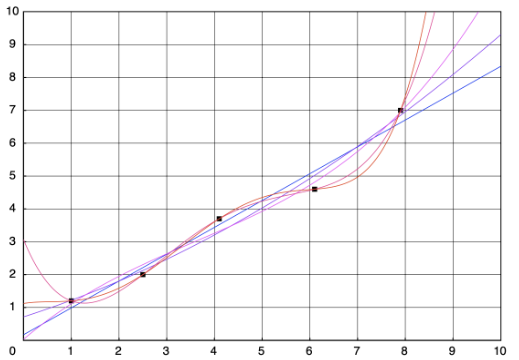
\includegraphics[width=10cm, scale=1]{images/overfitting}
	\caption{Overfitting}
	\label{overfitting}
\end{figure}


\subsection{Unsupervised Models}
L'apprendimento non supervisionato è una categoria di algoritmi di apprendimento automatico che utilizzano dati non etichettati per "imparare" da essi. In contrasto con l'apprendimento supervisionato, dove ci sono dati etichettati con le risposte corrette, l'apprendimento non supervisionato non ha accesso alle risposte corrette, ma cerca di scoprire relazioni o strutture all'interno dei dati.

Ci sono diverse tipologie di algoritmi di apprendimento non supervisionato, tra cui:
\begin{itemize}
\item Clustering: utilizzato per raggruppare gli esempi in base alle loro similitudini.
\item Riduzione della dimensionalità: utilizzato per ridurre la dimensionalità dei dati.
\item Analisi di componenti principali (PCA): utilizzato per individuare le componenti principali dei dati.
\item Apprendimento non supervisionato basato su reti neurali: utilizzato per apprendere rappresentazioni dei dati.
\item Anomaly detection: utilizzato per identificare dati anomali o fuori dalla norma.
\item Generative models: utilizzato per generare nuovi dati.


\end{itemize}
Nel rilevamento supervisionato delle anomalie, se vogliamo che un modello sia in grado di rilevare le anomalie, bisogna allenare il sistema in modo molto preciso sia nell' identificare sia il comportamento normale che quello anomalo.
Tuttavia, i comportamenti normali possono essere molteplici, così come i
comportamenti in presenza di anomalie e questo porta con se la necessità di fornire una grande quantità di dati etichettati per catturare piu comportamenti possibili. Purtroppo non e' sempre possibile in quanto le anomalie sono eventi rari e se il dataset di addestramento e' relativamente piccolo, anche il numero di anomalie non sara' sufficientemente grande, rendendo difficile la loro classificazione. 
Pertanto, l'apprendimento non supervisionato si adatta perfettamente al problema del rilevamento delle anomalie, poiché non è necessario etichettare grandi insiemi di dati. Inoltre, una parte delle anomalie derivano da nuovi comportamenti del sistema e per definizione, questi comportamenti non possono essere classificati correttamente con i metodi di rilevamento delle anomalie supervisionati senza effettuare prima un re-training.


\section{Model Evaluation}
La valutazione del modello è necessaria per quantificarne le prestazioni. La
scelta delle metriche e delle tecniche di valutazione dipende dal task di apprendimento come la classificazione o la regressione. 
In questa sezione ci si concentrerà sulle tecniche e sulle metriche più famose utilizzate per valutare la performance di un modello su un determinato compito.

\subsubsection{Tecniche}
\begin{itemize}
	\item \textbf{Random Split} genera in maniera casuale i tre insiemi di train, test e validazione. Il vantaggio di questo metodo è che c'è una buona probabilità che la popolazione originale sia ben rappresentata in tutti e tre gli insiemi, impedendo quindi un campionamento distorto dei dati.
	\item \textbf{Time Based Split} viene applicato sulle serie temporali in cui non e' possibile effettuare una suddivisione casuale dei dati in quanto si andrebbe a perdere informazioni come trend o seasonality. 
	      In questi casi, si utilizza una suddivisione temporale in cui, ad esempio, l'insieme di train può contenere i dati piu' vecchi, mentre quelli piu' recenti sono assegnati all'insieme di test. Per evitare l'overfitting introdotto da questo metodo, una variante a finestre di scorrimento e' preferibile: il modello viene allenato iterativamente piu' volte su una finestra temporale e valutato sulla parte restante dei dati, per poi allargare la finestra di training ad ogni iterazione (riducendo cosi quella di valutazione).
	\item \textbf{K-Fold Cross Validation} genera in modo casuale $k$ gruppi di dati ed iterativamente vengono usati $k-1$ gruppi per il training ed un gruppo per la valutazione.
	\item \textbf{Stratified K-Fold} e' simile al Cross Validation ma con la differenza che questo metodo tiene in considerazione la distribuzione delle classi dei dati, generando quindi gruppi con rateo simile al dataset originale.
\end{itemize}


\subsubsection{Metriche}
Alla base di tutte le metriche di valutazione vi e' la tabella di contingenza. Questa tabella permette di valutare le performance di un modello andando a relazionare, in piu modi, le predizioni di un modello con i dati di ground-truth.
La tabella \ref{contigency-table} mostra la struttura della tabella di contingenza.  La prima colonna contiene il numero delle predizioni positive fatte da un modello divise se queste sono effettivamente positive o negative. La seconda colonna funziona allo stesso modo ma per le predizione negative dello stesso modello. La terza colonna invece rappresenta la somma dei punti che sono realmente positivi e realmente negativi.
Riassumendo:
\begin{itemize}
\item True Positive: punti realmente positivi che sono predetti come tali
\item False Positive: punti realmente positivi ma predetti come negativi
\item False Negative: punti realmente negativi ma predetti come positivi
\item True Negative: punti realmente negativi che sono predetti come tali
\item Pos: Somma totale dei punti realmente positivi
\item Neg: Somma totale dei punti realmente negativi
\end{itemize}

\begin{table}[]
\centering
	\caption{\label{contigency-table}Tabella di contingenza}

\begin{tabular}{|l|l|l|l|}
\hline
                 & \textbf{Predizioni +} & \textbf{Predizioni -} & \textbf{Totale} \\ \hline
\textbf{Reale +} & TP                    & FP                    & Positivi        \\ \hline
\textbf{Reale -} & FP                    & TN                    & Negativi        \\ \hline
\end{tabular}
\end{table}

A questo punto e' possibile introdurre tutte le misure di performance:
\begin{itemize}
\item Accuracy: E' il rapporto tra i punti correttamente classificati rispetto al totale dei punti 
\[\frac{1}{|Te|} \sum_{x \in T_e} I[\hat{c}(x)=c(x)]\]
\item Error Rate: E' il rapporto tra i punti erroneamente classificati rispetto al totale dei punti, in breve \(1-accuracy\) 
\[\frac{1}{|Te|} \sum_{x \in T_e} I[\hat{c}(x)\neq c(x)]\]
\item True Negative Rate / Specificity: E' il rapporto tra i punti classificati correttamente come negativi rispetto al numero totale di punti realmente negativi
\[\frac{\sum_{x \in T_e} I[\hat{c}(x)=c(x)=-]}{\sum_{x \in T_e} I[c(x)=-]}\]
\item True Positive Rate / Recall: E' il rapporto tra i punti classificati correttamente come positivi rispetto al numero totale di punti realmente positivi
\[\frac{\sum_{x \in T e} I[\hat{c}(x)=c(x)=+]}{\sum_{x \in T_e} I[c(x)=+]}\]
\item Precision: E' il rapporto tra i punti correttamente classificati come positivi rispetto al numero di punti classificati come positivi
\[\frac{\sum_{x \in T_c} I[\hat{c}(x)=c(x)=+]}{\sum_{x \in T e} I[\hat{c}(x)=+]}\]
\item F-Measure Score: E' la media armonica tra precision e recall
\[F_\beta=\frac{\left(1+\beta^2\right) \cdot(\text { precision } \cdot \text { recall })}{\left(\beta^2 \cdot \text { precision }+\text { recall }\right)}\]
\end{itemize}

In generale non esiste una misura migliore e bisogna fare un'attenta valutazione su quale sia la preferibile rispetto al task da risolvere.
Ad esempio bisogna tenere in considerazione se c'e' una prevalenza di punti di una classe. Accuracy e' preferibile quando ci si aspetta una distribuzione equa delle classi. Quando i falsi-negativi non sono di interesse, ma lo sono i falsi-positivi, precision e' preferibile; al contrario quando i falsi-negativi sono molto importanti e non ci interessa dei falsi-positivi, recall e' la scelta corretta.
F-Measure invece e' necessaria quando si cerca un bilanciamento tra precision e recall dando importanza a entrambi i falsi-positivi ed i falsi-negativi. 
All'interno del contesto SKF e Anomaly Detection le anomalie sono sicuramente importanti da riconoscere e marcarle come negative, quindi falsi-negativi, potrebbe risultare in problemi alla linea di produzione. Ma allo stesso tempo un modello che produce molti più positivi di quanto deve risulterebbe in una perdita di fiducia da parte dell'operatore che inizierebbe semplicemente ad ignorare il feedback del modello in quanto produrrebbe soltanto falsi-positivi. Per questo motivo la scelta della metrica di valutazione e' ricaduta sulla F-Measure.



\section{Machine Learning Models}
In questa sezione vengono proposti diversi algoritmi e metodi di machine learning per l'Anomaly Detection, raggruppati per categoria.
I seguenti algoritmi sono implementati all'interno della libreria pubblica PyOD o TODS.

\subsection{Linear Models}
I modelli lineari sono un tipo di algoritmo di machine learning utilizzato per fare previsioni. Essi rappresentano la relazione tra le variabili indipendenti (chiamate anche caratteristiche) e la variabile dipendente (chiamata anche obiettivo) con una equazione lineare. La forma generale di un modello lineare è: 
\[ Y = B_0 + B_1X_1 + B_2X_2 + ... + B_n*X_n\]
dove $ Y $ è la variabile dipendente,  \(X_1, X_2, ..., X_n\)  sono le variabili indipendenti e \( B_0, B_1, B_2, ..., B_n\) sono i coefficienti del modello che vengono "appresi" dai dati.

\subsubsection{PCA}
La PCA è una riduzione lineare della dimensionalità che utilizza la Singular Value Decomposition dei dati per proiettarli in uno spazio dimensionale inferiore. Si tratta di spiegare la struttura di varianza-covarianza di una serie di variabili attraverso alcune nuove variabili che sono funzioni di quelle originali. Le componenti principali sono particolari combinazioni lineari delle \textit{p} variabili casuali  \(X1, X2, ..., Xp\) con tre importanti proprietà: (1) le componenti principali non sono correlate, (2) la prima componente principale ha la varianza più elevata, la seconda componente principale ha la seconda varianza più elevata e così via, e (3) la variazione totale in tutte le componenti principali combinate è uguale alla variazione totale delle variabili originali \(X1, X2, ..., Xp\). 
Queste componenti principali sono ottenibili da un'analisi agli autogeni della matrice di covarianza o della matrice di correlazione di \(X1, X2, ..., Xp\).
In questa procedura, la matrice di covarianza dei dati può essere decomposta in vettori ortogonali, detti autovettori, associati ad autovalori. Gli autovettori con alti autovalori catturano la maggior parte della varianza dei dati. Pertanto, un iperpiano a bassa dimensionalità costruito da \textit{k} autovettori può catturare la maggior parte della varianza dei dati. Tuttavia, gli outlier sono diversi dai punti di dati normali, cosa che è più evidente sull'iperpiano costruito dagli autovettori con autovalori piccoli.
Di conseguenza, i punteggi degli outlier possono essere ottenuti come la somma della distanza proiettata di un campione su tutti gli autovalori.

\subsubsection{K-PCA}
Kernel PCA e' un'estensione non-lineare di PCA. I dati di input sono mappati in uno spazio infinitesimale da cui KPA estrae le componenti principali. I tipi di kernel usati possono essere: lineare, polinomiale, sigmoidale o radiale.
\subsubsection{OCSVM}
Il metodo One Class Support Vector Machine (OCSVM) e' una versione derivata dalle Support Vector Machine al rilevamento di una sola classe. L'idea alla base consiste nel minimizzare l'iper-sfera contenente i punti di una singola classe e considerare tutti i punti esterni alla sfera come outliers.
La figura \ref{ocsvm} mostra un esempio del funzionamneto di ocsvm.
\begin{figure}[t]
	\centering
	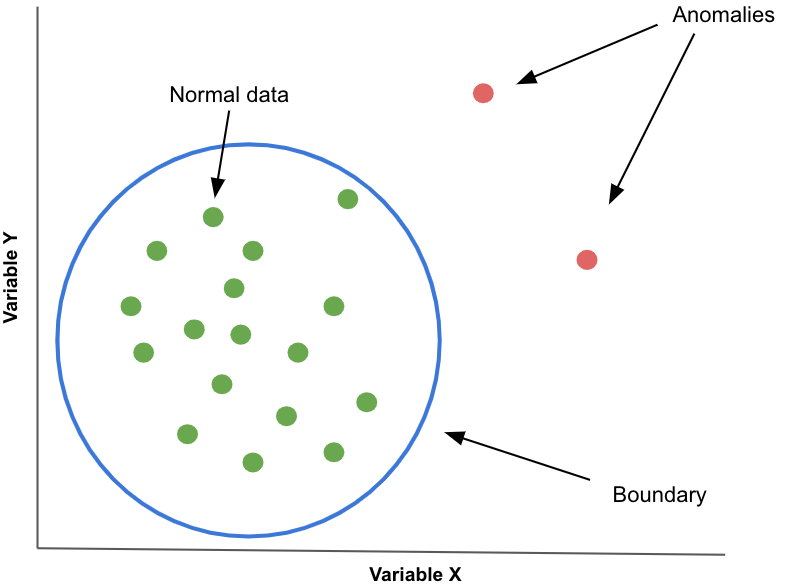
\includegraphics[width=10cm, scale=1]{images/ocsvm}
	\caption{OCSVM}
	\label{ocsvm}
\end{figure}


\subsubsection{AutoRegressive}
In un modello a regressione multipla viene fatto forecasting di una variabile di interesse attraverso una combinazione lineare di predittori. Un modello AutoRegressive, invece, viene fatto forecsting di questa variabile di interesse usand una combinazione lineare su \textit{valori passati} di questa variabile. Il termine auto-regressione indica una regressione della variabile fatta su se stessa.
Di conseguenza, un modello auto-regressive di ordine \textit{p} puo essere scritto come:
\[y_t=c+\phi_1 y_{t-1}+\phi_2 y_{t-2}+\cdots+\phi_p y_{t-p}+\varepsilon_t\]
dove $\varepsilon_t$ e' rumore bianco. Puo essere visto come una regressione multipla ma con valori ritardati di $y_t$ come predittori. 
La deviazione di un valore predetto rispetto a quello reale viene usato come outlier score.

\subsubsection{MCD}
Minimum Covariance Determinant (MCD) e' un metodo per stimare la media e la matrice di covarianza andando a minimizzare l'influenza delle anomalie. L'idea alla base e' quella di stimare questi valori andando a selezionare un sottoinsieme dei dati nel quale si spera non contengano anomalie.
Immaginando un approccio brute-force, l'algoritmo itera su ogni possibile sottoinsieme dei dati di una dimensione specifica. Vengono poi stimati la media e la matrice di covarianza per ogni sottoinsieme e poi vengono mantenute soltanto i valori per il sottoinsieme che ha il determinante della matrice di covarianza piu piccolo. Il motivo di questo e' perche il determinante di una matrice di covarianza indica quanto e' larga una distribuzione. Di conseguenza MCD cerca di minimizzare questo andando a prendere la distribuzione piu compatta. Questo consente di escludere le anomalie che saranno situate lontane dal resto dei dati.

\subsubsection{LMDD}
Linear Method for Deviation-based Outlier Detection (LMDD) impiega il concetto di Smoothing Factor il quale indica quanto puo essere ridotta la misura di dissimilarita andando a rimuovere un sottoinsieme degli elementi dal dataset. La funzione di dissimilarita puo essere qualsiasi misura di dispersione come la varianza, inter-quantile range, mediana ecc).
I punti che rimossi riducono maggiormente questa misura di dissimilarita possono essere valutati come anomalie.

\subsection{Distance Based Models}
I modelli non supervisionati basati sulla distanza sono una categoria di algoritmi che utilizzano la distanza tra i dati per scoprire relazioni e strutture nel dataset.

\subsubsection{KNN}
K-Nearest Neighbors (KNN) è un algoritmo di apprendimento supervisionato utilizzato per classificare oggetti in base alle loro proprietà. Dato un nuovo punto, l'algoritmo cerca i \textit{k} punti più simili (detti "vicini" o "neighbors") tra quelli già classificati e assegna all'oggetto in esame la classe più comune tra i \textit{k} vicini trovati. La scelta del valore di \textit{k} è un parametro importante del modello e può influire sulla sua accuratezza. In generale, un valore più alto di \textit{k} tende a ridurre la varianza del modello ma aumenta la sua bias.
Nel campo dell'Anomaly Detection, non e' di interessa assegnare la classe al punto in esame ma assegnare un punteggio di anomalia. Per un'osservazione, quindi, la sua distanza rispetto al \textit{k}-esimo punto piu vicino rappresenta lo questo score.

\subsubsection{DBSCAN}
BSCAN è un metodo di clustering che raggruppa i punti in aree ad alta densità e contrassegna i punti in regioni a bassa densità come anomali.
DBSCAN classifica quindi i punti in tre categorie. I punti centrali sono punti
contenenti almeno $minPts$ nel loro intorno definito da un parametro $\epsilon$. I border-point sono i punti che contengono almeno un punto centrale nel loro intorno, mentre gli altri punti sono considerati come rumore/anomalie. 
Per gestire serie temporali multivariate, DBSCAN considera ogni finestra temporale come un punto e il punteggio di anomalia è la distanza del punto dal cluster più vicino.

\subsubsection{LOF}
Local Outlier Factor (LOF) misura la deviazione locale di un dato punto rispetto ai suoi vicini. Sulla base del metodo dei K-nearest, la densità locale di questo punto viene valutata considerando la distanza rispetto ai suoi \textit{k} punti piu vicini. Il punteggio di anomalia viene invece calcolato confrontando la sua densità locale con quella dei suoi \textit{k} vicini più prossimi. Un punteggio elevato indica una densità inferiore a quella dei suoi vicini e quindi potenzialmente un'anomalia. Questo metodo è stato è stato applicato a serie temporali multivariate, dimostrando la sua capacità di individuare anomalie in dati a lungo termine
\begin{figure}[t]
	\centering
	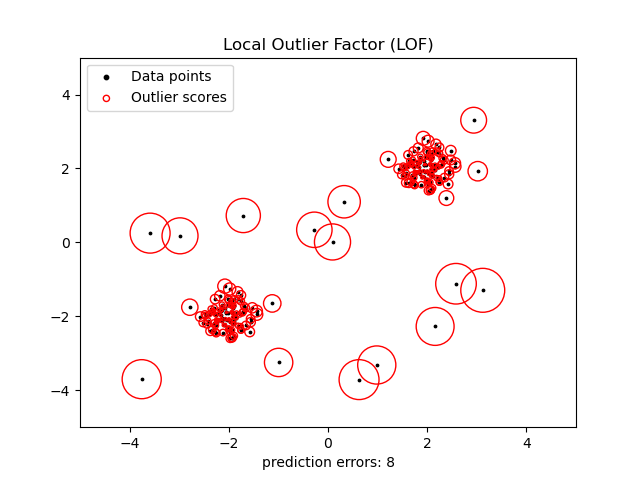
\includegraphics[width=10cm, scale=1]{images/lof}
	\caption{LOF}
	\label{lof}
\end{figure}

\subsubsection{COF}
Connectivity Outlier Factor (COF) e' un'evoluzione di LOF. Si basa sull'idea di assegnare un grado di anomalia ad ognuno dei punti, chiamato connectivty outlier factor.
Per ogni punto $x_i$, vengono selezionati i \textit{k} punti piu vicini e viene generato il percorso minimo che attraversi tutti i \textit{k} punti partendo da $x_i$. Infine COF viene calcolato andando a fare una media delle distanze di ogni percorso di $x_i$ verso i suoi \textit{k} punti piu vicini.

\subsubsection{CBLOF}
Cluster-Based Local Outlier Factor (CBLOF) e' anchesso un evoluzione di LOF.
Come primo step, CBLOF riceve in input i dati ed un algoritmo di clustering per andare a creare i cluster. Attraverso dei parametri va poi ha definire quale cluster viene considerato "grande" e quale viene considerato "piccolo". Vengono poi calcolati gli outlier score andando a considerare la dimensione del cluster a cui appartiene e la distanza piu vicina rispetto al centro di un cluster grande. Quindi piu un cluster di appartenenza e' piccolo e piu il punto e' lontano dal centro di un cluster grande, piu lo score di anomalia sara' alto. 

\subsubsection{HBOS}
Histogram based outlier detection (HBOS) e' un algoritmo di outlier detection che si basa sugli istrogrammi e assumendo indipendenza tra le feature. Per ogni feature computa il rispettivo istrogramma. Successivamente itera su ogni punti, se il valore di una feature di uno specifico punto $x_i$ rientra nella coda dell'istrogramma, questo punto vede alzarsi lo score di anomalia. Questo passaggio viene ripetuto rispetto ad ogni feature e su tutti i punti.

\subsubsection{SOD}
Subspace outlier detection (SOD) cerca di trovare gli outlier andando a considerare diversi sottoinsiemi dello spazio multidimensionale delle feature. Per ogni osservazione, SOD esplora il sottoinsieme delle dimensioni che si dirama parallalelamente dai punti vicini e determina quanto questa osservazione devia dai suoi vicini in questo sotto-spazio. 

\subsubsection{ROD}
Rotation-based Outlier Detection (ROD),  è un algoritmo privo di parametri che non richiede conoscenza sulla distribuzione dei dati e funziona in modo intuitivo nello spazio tridimensionale, dove i vettori 3D, che rappresentano i punti, vengono ruotati attorno alla mediana geometrica due volte in senso antiorario utilizzando la formula di rotazione di Rodrigues. I risultati della rotazione sono parallelepipedi i cui volumi vengono analizzati matematicamente come funzioni di costo e utilizzati per calcolare le Deviazioni Assolute Mediane e ottenere così il punteggio di anomalia. Per dimensioni elevate > 3, il punteggio complessivo viene calcolato prendendo la media dei punteggi complessivi dei sottospazi 3D risultanti dalla scomposizione dello spazio dati originale.


\subsection{Probabilistic Models}
I modelli probabilistici non supervisionati sono una categoria di algoritmi che utilizzano la probabilità per descrivere e generare i dati. Essi utilizzano una distribuzione di probabilità per rappresentare la relazione tra le variabili del dataset.
\subsubsection{KDE}
Kernel Density Estimation (KDE) e' l'applicazione di un "kernel smoothing" per la stima della probabilita. 
Siano $(X_1,...,x_n)$ osservazioni indipendenti e identicamente distribuite prese da una distribuzione univariata con una densita non conosciuta \textit{f} per qualasiasi punto \textit{x}. Siamo interessati nello stimare la forma di questa funzione \textit{f}. La funzione kernel di stima e':
\[\widehat{f}_h(x)=\frac{1}{n} \sum_{i=1}^n K_h\left(x-x_i\right)=\frac{1}{n h} \sum_{i=1}^n K\left(\frac{x-x_i}{h}\right)\]

Dove \textit{K} e' il kernel, una funzione non negativa, e $h>0$ e' un parametro di smoothing chiamato bandwidth. Un kernel con pedice $h$ e' chiamato \textit{kernel scalato} ed e' definito da: $Kh(x) = 1/h K(x/h)$. 
Il valore di $k$ deve essere scelto tenendo conto del trade-off bias/variance.
I kernel piu utilizzati sono: uniforme, triangolare, normale e altri.
Le stime di densita con kernel sono fortemente correlate agli istrogrammi, ma sono dotati di proprieta di smoothing o di valori continui usando appunto questi kernel.
La figura \ref{kde_model} mostra un confronto tra un istogramma con una funzione di stima di densita con kernel.
L'applicazione di questo modello nell'Anomaly Detection avviene andando a generare, per un'osservazione, uno score di anomalia corrispondente al valore negativo del logaritmo della probabilita di densita.

\begin{figure}[t]
	\centering
	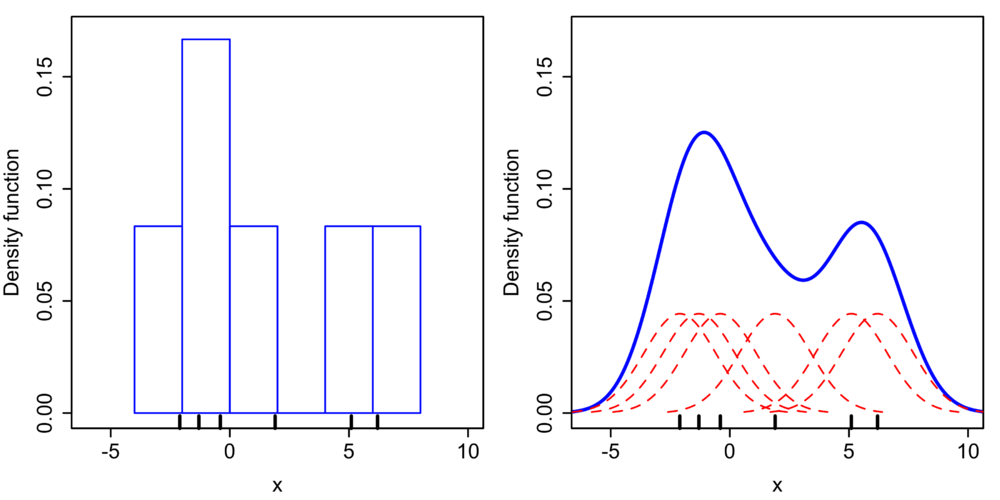
\includegraphics[width=10cm, scale=1]{images/kde_model}
	\caption{KDE}
	\label{kde_model}
\end{figure}


\subsubsection{GMM}
I GMM sono una generalizzazione delle distribuzioni gaussiane e possono essere utilizzati per rappresentare qualsiasi serie di dati che possono essere raggruppati in più distribuzioni gaussiane. GMM è un modello probabilistico che presuppone che tutti i punti dati siano generati da una insieme di distribuzioni gaussiane con parametri sconosciuti e può essere utilizzato per il clustering, oppure per stimare la probabilità che un nuovo punto dati appartenga a ciascun cluster. Sono anche relativamente robusti agli outlier, il che significa che possono fornire risultati accurati anche se ci sono alcuni punti di dati che non si adattano perfettamente a nessuno dei cluster. Ciò rende i GMM uno strumento flessibile e potente per la clusterizzazione dei dati. Può essere inteso come un modello probabilistico in cui si ipotizzano distribuzioni gaussiane per ciascun gruppo, con medie e covarianze che ne definiscono i parametri.

Per la stima di questi parametri si esegue l'algoritmo di Expectation-Maximization chiamato cosi in quanto vengono alternate iterativamente due fasi: quella di excpectation e quella di maximization. L'algoritmo parte inizializzando prima i parametri del GMM. A ogni iterazione, la fase di expectation calcola il valore atteso della funzione log-likelihood rispetto ai parametri correnti. Questa valore viene poi utilizzato per massimizzare la log-likelihood nella fase di massimizzazione.

E' possibile adottare questo modello nell'Anomaly Detection allenandolo rispetto ad un set di dati e poi assegnando un punteggio ai nuovi punti: quelli significativamente diversi dal resto dei dati verranno marcati come anomalia.

\subsubsection{ABOD}
Angle Based Outlier Detection (ABOD) si basa sull'idea di osservare l'angolo formato da un insieme di tre punti qualsiasi nello spazio delle feature multivariate. La varianza dell'ampiezza dell'apertura angolare risulta diversa per i punti anomali e per quelli normali: la varianza osservata è più alta per i punti inlier e piu bassa per gli outlier, quindi tale misura puo essere usata per separare punti normali da outlier. ABOD funziona abbastanza bene nello spazio ad alta densità, a differenza di altre misure basate sulla distanza che soffrono della "curse of dimensionality" in quanto gli angoli possono fornire una rappresentazione migliore della vicinanza.
\begin{figure}[t]
	\centering
	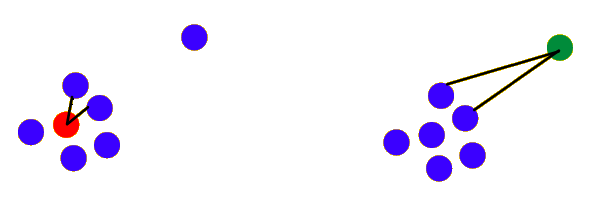
\includegraphics[width=10cm, scale=1]{images/abod}
	\caption{ABOD}
	\label{abod}
\end{figure}
Un'esempio sull'idea alla base di ABOD e' presente in figura \ref{abod}.
Considerando il punto rosso come pivot, viene calcolato l'angolo racchiuso tra questo punto e qualsiasi altro punto dello spazio e con molta probabilita si notera' un'altra varianza tra questi valori. Questo andamento indica che il punto pivot fa parte di un cluster ad alta coesione.
Se si considera come pivot invece il punto verde e procedendo con gli stessi calcoli per ogni coppia di punti, la varianza angolare sara' molto piu bassa, indice che quel punto e' molto probabilmente un outlier.

\subsubsection{ECOD}
Empirical-Cumulative-distribution-based Outlier Detection (ECOD) e' un modello probabilistico che basa il suo funzionamento nel calcolare, per ogni punto $x_i \in X$, la probabilita che esista un punto almeno "estremo" come $x_i$.
ECOD prima stima la distribuzione dei dati di input senza l'ausilio di parametri esterni andando a computare la distribuzione cumulativa empirica per ogni dimensione del dataset. Successivamente usa la distribuzione empirica per stimare la probabilita, su ogni dimensione, per ogni punto. Infine computa lo score di anomalia di ognuno dei punti andando ad aggregare le stime di probabilita su tutte le dimensioni.

\subsubsection{COPOD}
Copula Based Outlier Detection (COPOD) si ispira alla copula per modellare la distribuzione dei dati multivariati. Costruisce dapprima una copula empirica e la utilizza per predire la tail-probability di ogni punto per determinare il suo
livello di "estremita". Intuitivamente, si puo pensare a questo come a calcolare
un valore p-anomalo.

\subsubsection{SOS}
Stochastic Outlier Selection (SOS) utilizza il concetto di affinità per quantificare la relazione tra un punto e un altro. L'affinità è proporzionale alla somiglianza tra due punti di dati. Quindi un punto ha poca affinità con un punto dati dissimile. 
Un'osservazione viene classificata come outlier quando tutti gli altri punti hanno un'affinità insufficiente con esso.

\subsubsection{Sampling}
Fast-KNN andando a scegliere a caso un sottoinsieme di punti per fare knn-distance. cosi non li computo tutti 
https://pdfs.semanticscholar.org/6e3b/d9d74747af4c7ea0c98e339c0b488cac844d.pdf

\subsection{Ensemble Models}
\subsubsection{I-Forest}
\#TODO
\subsubsection{INNE}
\#TODO
\subsubsection{Feature Bagging}
\#TODO

\section{Neural Network Models}
\subsection{Deep}
\subsubsection{DeepSVDD}
\#TODO
\subsection{Auto Encoders}
autoencoders
\#TODO
\subsubsection{Variational Autoencoders}
\#TODO
\subsection{LSTM}
lstm
\subsubsection{telemanom}
\#TODO
\subsubsection{DeepLog}
\#TODO

\subsection{Adversarial Networks}
\subsubsection{Anogan}
\#TODO
\subsubsection{ALAD}
\#TODO

\subsection{Graph Based}
\subsubsection{LUNAR}
\#TODO
\section{Thresholding}
\subsection{IQR}
\#TODO
\subsection{Z-Score}
\#TODO
\subsection{yGMM}
\#TODO